\chapter{Domain Name System}
\section{Overview}
This section will describe the technological fundamentals of DNS, as well as related technologies like IP addressing. The technologies will be described along with example software used to display different parts of the theory.

The section will also contain a description of the BIND DNS software, along with installation and user guide. 

This section will not focus on the chosen real-life case. This is a general description of the technology.
\section{IP Addressing}
\subsection{IP overview}
To access any resource on the internet (or LAN), be it a website or a specific device, a location is needed. When dealing with internet-related technologies, this location is specified by an \textit{IP address}. 

On any given network, an IP address should be unique to a specific device/server. However, local network routers generally have a private block of IP addresses for devices on that specific sub-net and a separate IP for the outside world (access to sub-net devices are forwarded to the specific devices by the router).
The router then acts as the \textit{gateway} to the outside world and should be accessible by an IP within the range of the sub-net.

To check the IP address of a device, the tool ifconfig (Linux) or ipconfig (windows) can be used

\begin{figure}[h!]
	\centering
	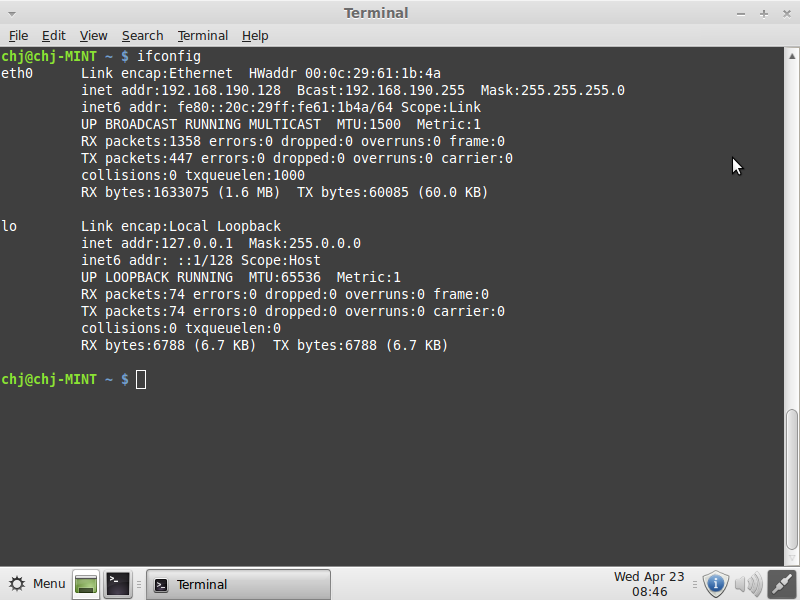
\includegraphics[width=\textwidth]{ifconfig.png}
	\caption{ifconfig from Linux machine}
\end{figure}


If the tool \textit{nm-tool} is run (on a Linux machine) the output will look like this:

[Insert picture of nm-tool]

Where 

\textbf{Address} 
Denotes the machines' IP on the local sub-net. Other devices on the sub-net will use this IP on to communicate with the device.

\textbf{Prefix} 
Denotes the subnet - mask of the network. This shows how many individual addresses are available on the sub-net. An IP address is 32 bits total and in the \textit{xx.xx.xx.xx/yy} format, \textit{yy} denotes the amount of bits reserved for the address of the \textit{subnet} and not the address of the individual devices on the net. Thus, a subnet with fewer bits reserved for the subnet address (say, 16 bits) can contain more individual addresses. This can be utilized in a larger sub-net, containing smaller sub-nets with the individual devices and thus fanning out to the individual addresses. 

\textbf{Gateway}
As explained above, most devices are connected to a sub-net, where their address only has to be individual on the sub-net. The \textit{gateway} then, is the point of access to the outside world. This could be the main router, of the subnet. All access to the internet goes through this device and the Gateway field, obtained when running nm-tools, describes the address of this device. 

\textbf{DNS}
Tells us the address of the first DNS server, we will query for an address of a resource on the internet. When a user types the URL of a website, e.g. www.google.com, this IP address is queried for the actual address of the URL, this is explained in detail further into this report.


\section{Name Resolution and forwarding}
Name resolution is what DNS is all about. It is the concept of mapping a name to something else, in this case a domain name to an IP address. A domain name is is build from a number of pieces that is used to resolve the name. First there's the root, a ., then the top level domain ex dk, com, se, then a number of hostnames. Each of these parameteres are used to resolve which IP address they are associated with by going through a number of DNS resolution servers in ether an iterative or recursive way.

By using name resolution are we able to use some more human memorable domain names than the hard to remember IP addresses, that are smart for use in computer science.

In DNS forwarding is used to access domains outside of your local network ex to access webpages on the internet. A forwarder is also able to use caching to make DNS resolution faster.
\subsection{Iterative}
As explained above, the DNS server resolves the IP address of a specified resource. This can be done iteratively and recursively.
When resolving an IP address iteratively, the largest burden of work is transferred to the requester. 
When a DNS query reaches the server, the server will check if it has the address cached/knows the address of the URL. If it does not, the server will transmit back the address of the next DNS server in the hierarchy until the root domain is reached.
Thus, the requester must then query the next DNS server and so on until a server is reached, which knows the address of the requested url.

All DNS servers \textbf{must} implement Iterative queries.

\subsection{Recursive}
With recursive address resolution, the burden of work is on the DNS server. When the server is queried and it does not have the IP cached/know the IP, the server will then forward the request to the next server in the hierarchy. The query will then be answered iteratively or recursively by the next server and so on, until the correct address is found.
The server then waits until it gets the correct address and \textit{then} returns the address to the original requester. The original requester will then only have to do \textit{one} request and does not need to know anything about the further process. 

\subsection{Caching}
%Why is this important?
%How does it help in Recursive/iterative resolution.
Caching of DNS lookups can be done in a few different ways. Closest to the user and the fastest is local caching which can be done with a DNS server like BIND. It is a local server that saves name resolutions for that webpages you have visited and therefore is able to make the resolution a lot faster.

Then there is caching on the non-local DNS servers. This is very smart for a recursive DNS address resolution because all resolutions goes through the root server and it makes it able to cache all the most used pages. In interative DNS resolutions the server is only able to cache a part of the lookup because it will never get the result of the whole lookup.

\subsection{Security [DNSSEC]}
\section{BIND}
\subsection{Downloading}
\subsection{Configuration}
\subsection{Basic Use}
The most basic use of BIND is to set up DNS caching, so that the first time you visit a domain BIND will cache the result and use that the next time you visit that domain.
BIND does also have way more advanced features and is therefore the most widely used DNS server in both large and small scale.

%This chapter should contain an in-depth description of the technology,
%i.e. DNS, DDS, or RMI. You should at least address
%\begin{itemize}
%\item The purpose of the technology
%\item Technology alternatives
%\item Downloading, installing, configuring, and employing the technology
%\end{itemize}
